
\newpage
\thispagestyle{empty}
\mbox{}
\chapter{Sistema de manera global}
\label{ch:chapter2}

\section{Modelo para la simulación} \label{Simulacion_Modelo}

Antes de describir cada uno de los algoritmos pertenecientes al sistema se va a definir la función gaussiana utilizada para la simulación de la radiación de la fuente de contaminación.

\begin{equation} \label{Funcion_Gaussiana} 
	f\left(x,y\right) = p\cdot{e}^{-\left(x-c_o\right)^{T}\cdot{M}\cdot\left(x-c_{o}\right)}
\end{equation}

Donde $x=\left(x,y\right)$, $c_o=\left(x_{o},y_{o}\right)$ sería la posición del centro de la gaussiana. Además, 

\begin{equation}
	\begin{aligned}
	M= 	
	\begin{bmatrix}
		\frac{\cos^{2}{\theta}}{2\cdot{\sigma^{2}_{x}}}+ \frac{\sin^{2}{\theta}}{2\cdot{\sigma^{2}_{y}}} & \frac{\sin{2\cdot\theta}}{4\cdot{\sigma^{2}_{x}}}+ \frac{\sin{2\cdot\theta}}{4\cdot{\sigma^{2}_{y}}}\\\\
		
		\frac{\sin{2\cdot\theta}}{4\cdot{\sigma^{2}_{x}}}+ \frac{\sin{2\cdot\theta}}{4\cdot{\sigma^{2}_{y}}} & \frac{\sin^{2}{\theta}}{2\cdot{\sigma^{2}_{x}}}+ \frac{\cos^{2}{\theta}}{2\cdot{\sigma^{2}_{y}}}\\
	\end{bmatrix}
	\end{aligned}
\end{equation}

Es una matriz definida positiva y proviene de $R\cdot{S}\cdot{R}^{T}$ con $R$ siendo la matriz de rotación ordinaria en 2D para un ángulo $\theta$ definiéndose a $S$ como:

\begin{equation}
		\begin{aligned}
	S= 	
	\begin{bmatrix}
		\frac{1}{2\cdot{\sigma^{2}_{x}}} & 0\\\\
		0 & \frac{1}{2\cdot{\sigma^{2}_{y}}}\\
	\end{bmatrix}
	\end{aligned}
\end{equation}

En donde, $\sigma^{2}_{x}$ con $\sigma^{2}_{y}$ serían a desviación típica de la gaussiana con los ejes x e y respectivamente.

\begin{figure}[htb]
  \begin{center}
    \subfigure[Función definida en 3D]{
        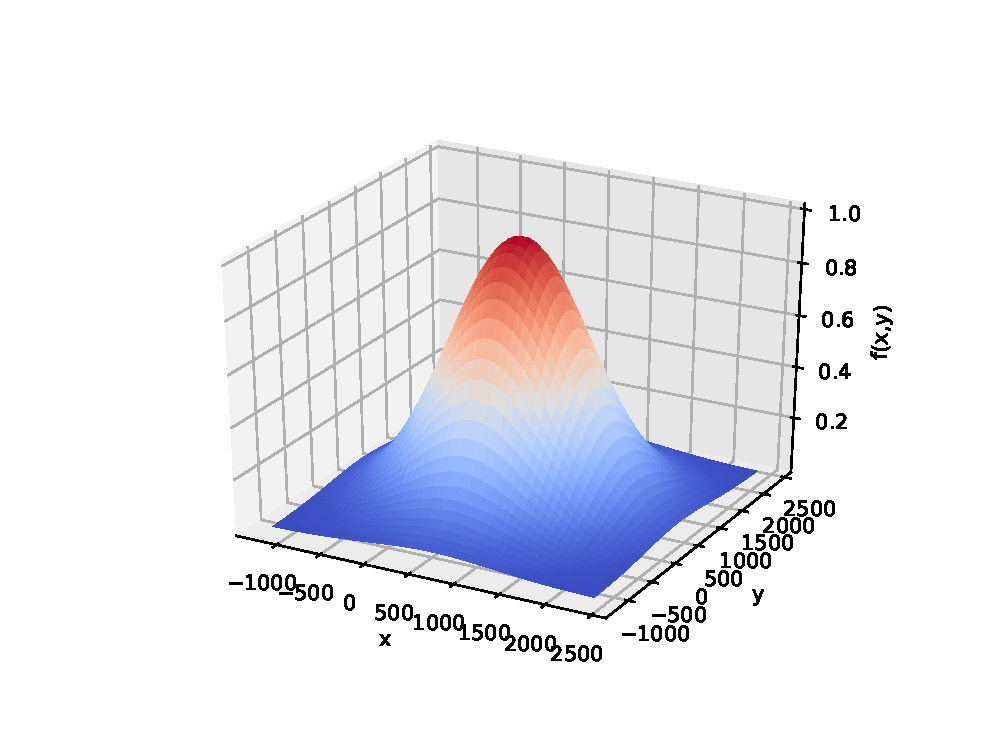
\includegraphics[width=0.45\textwidth]{figures/Gaussiana.eps}
        \label{Fgauss}}
    \subfigure[Curvas de nivel]{
        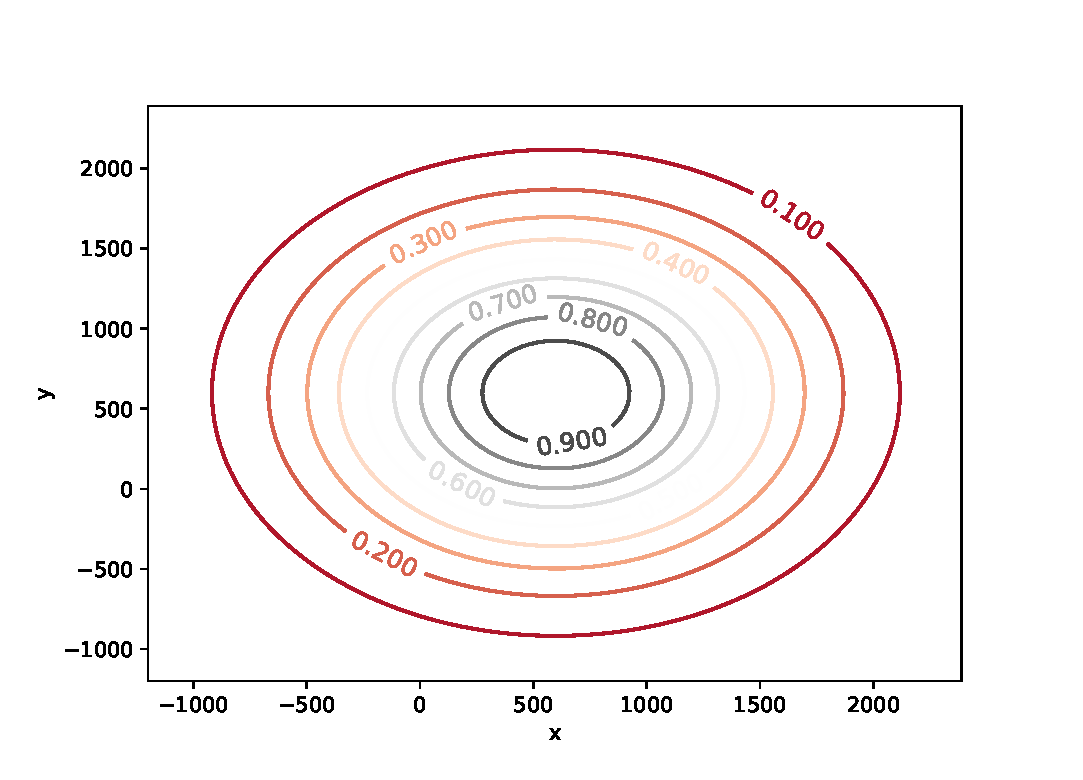
\includegraphics[width=0.45\textwidth]{figures/CurvasNivelGauss.eps}
        \label{CurvasGauss}}
    \caption{Representación de una función gaussiana}
    \label{FunGauss}
  \end{center}
\end{figure}


Se puede particularizar a un caso más sencillo para facilitar el análisis del rendimiento del sistema de la siguiente forma:

\begin{itemize}
	\item Normalizar el volumen encerrado debajo de la gaussiana para que este tenga un valor unitario. Esto se obtiene definiendo a $p=\frac{1}{2\cdot{\pi}\sigma_{x}\sigma_{y}}$.
	\item Presentar desviaciones iguales en ambos ejes $\sigma_{x}=\sigma_{y}=\sigma$.
\end{itemize}

Con estas dos consideraciones la expresión final sería:

\begin{equation}
	f\left(x,y\right)=\frac{1}{2\cdot{\pi}\cdot{\sigma^{2}}}e^{\frac{\left(x-x_{o}\right)^{2}+\left(y-y_{o}\right)^{2}}{2\cdot{\sigma^2}}}
\end{equation}

Esta representación es la que posteriormente se usará para las diferentes simulaciones aportadas en el capítulo \ref{ch:chapter3}. 

\section{Algoritmo de estimación de gradiente para la búsqueda de fuentes} \label{Estima}

Anteriormente se discutió que el objetivo del algoritmo es la búsqueda de fuentes, basándose en mediciones locales de múltiples robots situados de manera simétrica en un espacio de 2D. En dicho procedimiento, se consideran N robots distribuidos uniformemente a lo largo de una formación circular con un radio D y un punto central c definido en dos dimensiones, tal como se muestra en la siguiente figura: \\

\begin{figure}[htb]
\centering
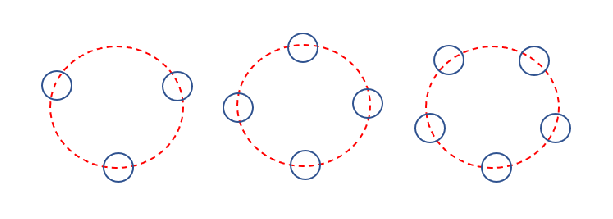
\includegraphics[width=0.95\textwidth]{figures/Disposicion_Robots.eps}
\caption{Disposición de los agentes en torno a la formación circular.} \label{Disp:Robots}
\end{figure}

Adicionalmente, cada uno de los agentes deberá tener la capacidad de medir la intensidad de la señal mediante un sensor. En términos matemáticos, la distribución de la señal es una función espacial bidimensional que representa un campo escalar con un máximo o mínimo definido justo en la posición donde dicha fuente se localiza. Por lo tanto, se va a considerar que la señal es emitida por una única fuente de modo que su punto critico en $z_*$ es el único máximo definido del campo escalar.

Para la obtención del gradiente, se adoptan los \textbf{algoritmos de tipo consenso} siendo estos un mecanismo que permite a maquinas coordinarse en un entorno distribuido, es decir, encuentran la solución al problema de la comunicación entre diferentes entes aislados con el objetivo de ponerse de acuerdo para realizar una tarea concreta.

Se define una función $f\left(x\right)$ con $x\in\mathbb{R}^{n}$, además de ser continua y derivable para todo x. Aplicando el desarrollo en serie de Taylor para un valor de $n\geq{2}$ se tiene:

\begin{equation}\label{TaylorNormal}
	f\left(x\right)=f\left(x_{*}\right)+\mathrm{\nabla}{f}{\left(x_{*}\right)}^{T}\left(x-x_{*}\right)+\frac{1}{2!}\cdot{\left(x-x_{*}\right)}^{T}\cdot{H}\left({f}\left(x_{*}\right)\right) 		\cdot\left(x-x_{*}\right)+O\left(x_{*}^3\right)
\end{equation}

Donde:

\begin{equation*}
	\begin{aligned}
		\mathrm{\nabla}{f}=
	\begin{bmatrix}
		\frac{\partial{f}}{\partial{x}_1} \\
		\frac{\partial{f}}{\partial{x}_2}  \\
		\vdots \\
		\frac{\partial{f}}{\partial{x}_n}
	\end{bmatrix}
	\end{aligned}
	\qquad\text{y}\qquad
	\begin{aligned}
	{H}\left(f\right)=\mathrm{\nabla}^{2}{f}= 	
	\begin{bmatrix}
		\frac{\partial^{2}{f}}{\partial{x}_{1}^{2}} & \frac{\partial^{2}{f}}{\partial{x}_{1}\cdot\partial{x}_{2}} & \cdots & \frac{\partial^{2}{f}}{\partial{x}_{1}\cdot\partial{x}_{n}}\\
		\frac{\partial^{2}{f}}{\partial{x}_{2}\cdot\partial{x}_{1}} & \frac{\partial^{2}{f}}{\partial{x}_{2}^{2}} & \cdots & \frac{\partial^{2}{f}}{\partial{x}_{2}\cdot\partial{x}_{n}}\\
		\vdots & \vdots & \ddots & \vdots\\
		\frac{\partial^{2}{f}}{\partial{x}_{n}\cdot\partial{x}_{1}} & \frac{\partial^{2}{f}}{\partial{x}_{n}\cdot\partial{x}_{2}} & \cdots & \frac{\partial^{2}{f}}{\partial{x}_{n}^{2}}
	\end{bmatrix}
	\end{aligned}
\end{equation*}

Para evaluar el punto máximo de concentración lo que interesa es que $\mathrm{\nabla}{f}{\left(x_{*}\right)}=0$. No obstante, en el problema en cuestión no se dispone de información sobre dicho gradiente solo se tienen las medidas tomadas por los sensores en cada uno de los vehículos es por ello que se va a aprovechar para realizar una estimación del gradiente en el centro del círculo $\hat{\nabla}{f}\left(c\right)$.

\begin{figure}[htb]
\centering
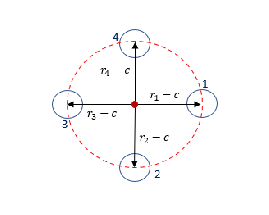
\includegraphics[width=0.5\textwidth]{figures/p3.eps}
\caption{Estrategia colaborativa para el cálculo del gradiente en el centro de la circunferencia formada por los agentes.} \label{Estrategia_Colaborativa}
\end{figure}

Particularizando para una distribución uniforme a lo largo de un circulo con radio D, un ángulo de rotación $\phi_o\left(t\right)=w_o\cdot{t}$, en el que los agentes se mueven con velocidad angular  y el centro de la formación c. 

\begin{equation*}
	r_i = c + D\cdot{R}_{\theta_i}\cdot{e}\hspace{10mm}{i = 1,...,N}
\end{equation*}

En donde, $r_{i}$ es la posición del robot i con respecto al radio del circulo, ${\phi }_{i}=\phi_{o}+\frac{2\cdot\pi\cdot{i}}{N}$ es el ángulo de rotación, $R_{\phi }$ es la matriz de rotación definida como $\left[ \begin{array}{cc} {c}_{\phi } & -{s}_{\phi } \\  {s}_{\phi } & {c}_{\phi } \end{array} \right]$ y  $e\ =\ {\left[1,0\right]}^T$.\\


A partir de la ecuación \ref{TaylorNormal} pero haciendo la expansión de Taylor hasta el termino primer orden sobre cada una de las medidas $f\left(r_i\right)$ en torno al punto c y redefiniendo a $D$ como $D=||r_i-c||$, se obtiene:

\begin{equation} \label{PuntoPartidaGradiente}
	f\left(r_i\right)-f\left(c\right)=\nabla{f\left(c\right)}^T\left(r_i-c\right)+\varphi_i\left(D,c\right)\hspace{12mm}\forall{i},\cdots,N
\end{equation}

En donde, $\varphi_i\left(D,c\right)$ denota el remanente de la expansión de Taylor. 

Se podría estimar el gradiente en el centro $c$ si se conociera el valor de la función $f\left(c\right)$. Sin embargo, es posible obtener una aproximación para el gradiente empleando directamente las medidas tomadas por los sensores de cada uno los agentes $f\left(r_i\right)$ de la siguiente forma:

\begin{equation}\label{Fun_Esti}
	\frac{2}{N\cdot{D}^2}\cdot\sum_{i=1}^{N}f(r_{i})\cdot(r_{i}-c)=\underbrace{\nabla{f}\left(c\right) + \varphi\left(D,c\right)}_{:=\hat{\nabla}{f}\left(c\right)}
\end{equation}

La obtención de dicha expresión, así como la prueba de su validez pueden encontrar en \cite{Estimacion_Gradiente} y \cite{Adicional_Estimacion_1}. En donde, $\varphi\left(D,c\right)$ es el error de la aproximación. 
\newpage
Para evaluar la fiabilidad de la estima se va a comparar con el valor exacto del gradiente obtenido sobre la función gaussiana y como influye en la bondad de dicho cálculo el número de agentes empleados y el radio del círculo de la formación.

Por ello, se establece una posición arbitraria para el centro de la formación  se encuentre relativamente lejos de la fuente y así evaluar la variación del número de agentes con un radio unitario y del radio con el mínimo de número de agentes posibles.

Finalmente, se hace uso de \ref{Funcion_Gaussiana} cuyos valores serían $c_{o}=[0,0]$, el ángulo $\theta$ nulo, una desviación uniforme en ambos ejes $\sigma_{x}=\sigma_{y}=\frac{1}{1000}$ para que la matriz quede definida como $S = \bigl[\begin{smallmatrix}\frac{1000}{\sqrt{2}} & 0\\ 0 & \frac{1000}{\sqrt{2}}\end{smallmatrix}\bigr]$  y cuyo volumen es $p = 1$.

\begin{figure}[htb]
  \begin{center}
    \subfigure[N = 2]{
        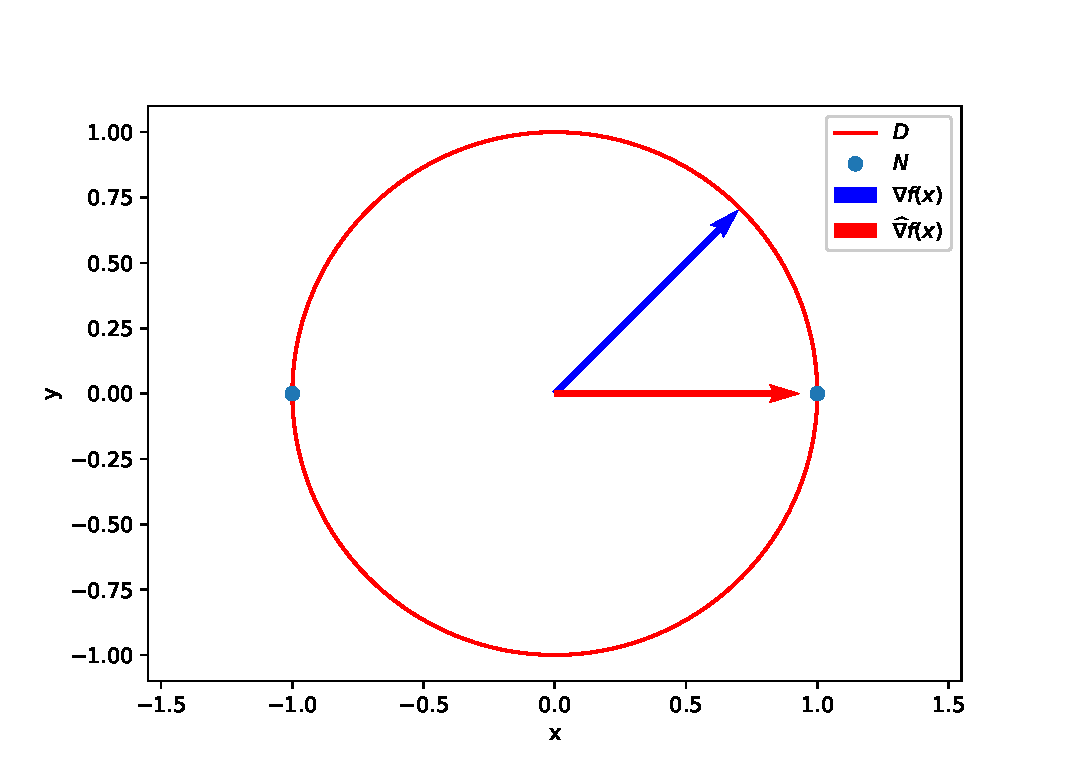
\includegraphics[width=0.40\textwidth]{figures/N2_RFIJO.eps}
        \label{N = 2}}
    \subfigure[N = 3]{
        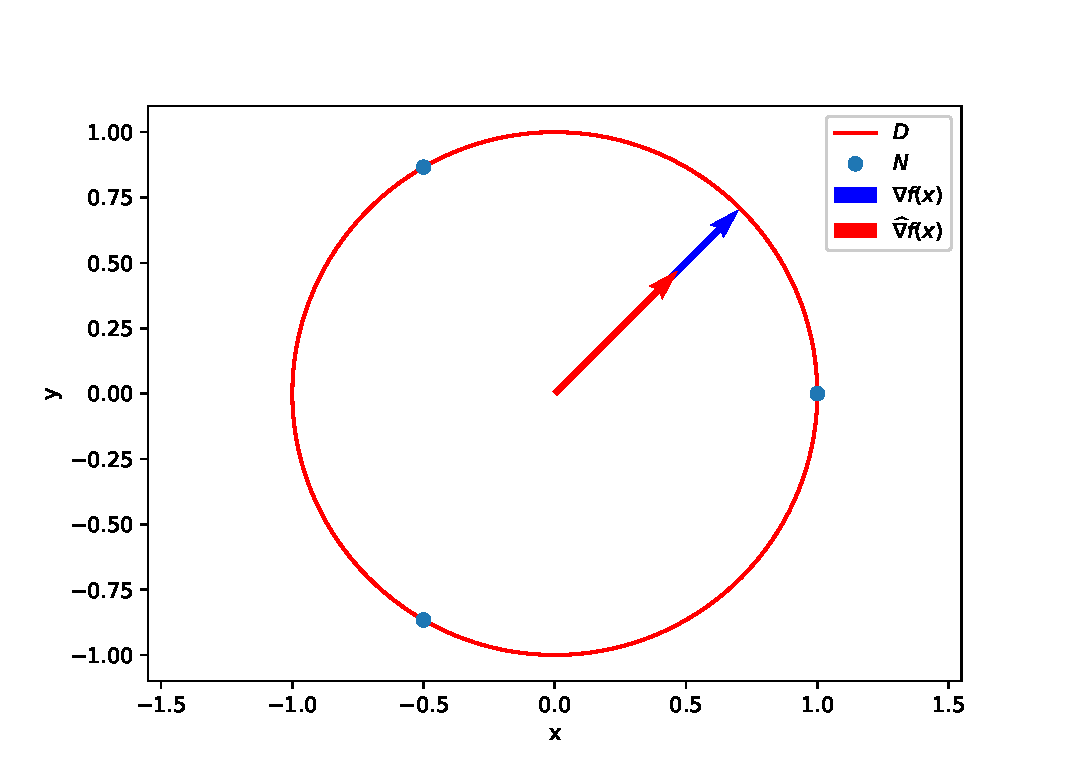
\includegraphics[width=0.40\textwidth]{figures/N3_RFIJO.eps}
        \label{N = 3}}
    \caption{Estimación del gradiente en función del número de agentes con D = 1}
    \label{NAGENTSEST}
  \end{center}
\end{figure}

Se observa en la figura que al aumentar el número de agentes llega un punto donde el error es prácticamente despreciable. Por otra parte, el algoritmo solo funciona si cooperan tres o mas vehículos, tal como se anticipaba en \cite{Estimacion_Gradiente}. De manera análoga, se procede a evaluar el efecto del radio:

En el caso de \ref{VARD} la relación es inversa al número de agentes, es decir, cuanto menor es el radio menor será el error. No obstante, se deben considerar las dimensiones de los vehículos dado que si el radio es excesivamente pequeño pueden generarse colisiones entre ellos.

\begin{figure}[htb]
  \begin{center}
    \subfigure[D = 100]{
        \includegraphics[width=0.40\textwidth]{figures/R100_NFIJO.eps}
        \label{D = 100}}
    \subfigure[D = 10]{
        \includegraphics[width=0.40\textwidth]{figures/R10_NFIJO.eps}
        \label{D = 10}}
    \caption{Estimación del gradiente en función del radio del círculo con N = 3}
    \label{VARD}
  \end{center}
\end{figure}

Finalmente, para un estudio más detallado del resto de parámetros y sus respectivos efectos sobre la estimación del gradiente, se debe discutir antes la importancia que tiene la coordinación de estos en torno a la formación circular.

\section{Algoritmo de control de formación circular}

El control de la formaciones tiene como objetivo conseguir que un sistema formado por múltiples vehículos naveguen manteniendo una forma geométrica deseada. Una forma particular de hacerlo es mediante algoritmos de cooperación entre los agentes.

El modelo dinámico que se utilizará considera vehículos tipo monociclo con velocidad constante, es decir, solo se actúa sobre la dirección del vehículo a través de giros coordinados actuando sobre el ángulo de orientación. Definiéndose como objetivo el describir un \textbf{algoritmo distribuido para controlar formaciones circulares} aplicados a los USVs comentados en \ref{Motiv}. Estos tendrán velocidades constantes y se actuará sobre la velocidad angular que poseen en torno a un punto central. 
\newpage
Es importante destacar que el algoritmo va a tener dos tareas:

\begin{itemize}
	\item Inicialmente cada uno de los vehículos estarán en posiciones arbitrarias y deberán converger hacia la formación circular definida en torno a un punto central conocido.
	\item Posteriormente, han de distribuirse uniformemente en torno a dicha formación. Esto será posible al minimizar el error existente entre sus ángulos como más adelante se comentará.
\end{itemize}

No obstante, para ambos casos se tiene que tomar en cuenta la manera de comunicarse entre los agentes que se describe a continuación. 

Inicialmente, se considera una formación con $N\geq{2}$ vehículos cuyas posiciones $p$ se definen por $p_i\in\mathbb{R}^2$ con $i\in\left\lbrace{1,\cdots,N}\right\rbrace$, en donde los vehículos son capaces de detectar las posiciones relativas con respecto a sus vecinos. Evaluando la relación existente entre los vecinos ésta puede describirse mediante un grafo $\mathbb{G}=\left(\mathcal{V},\mathcal{E}\right)$ siendo $\mathcal{V}=\left\langle{1,\cdots,N}\right\rbrace$ los distintos nodos pertenecientes al grafo, en donde cada uno de ellos representa un vehículo y $\mathcal{E}\subseteq\mathcal{V}\times\mathcal{V}$ sus aristas. El conjunto de los vecinos del vehículo $i$ esta definido por $\mathcal{N}_i\triangleq\left\lbrace{j\in\mathcal{V}:\left(i,j\right)\in\mathcal{E}}\right\rbrace$. Dos vértices son adyacentes si $\left(i,j\right)\in\mathcal{E}$. Un camino desde el nodo $i$ hasta el nodo $j$ es una secuencia que comienza en $i$ y termina en $j$, de manera que dos vértices consecutivos son adyacentes, y si $i=j$ el camino se le conoce como ciclo. \cite{Control_Formacion}

Asumiendo que el grafo $\mathbb{G}$ esta conectado, es decir, existe un camino que conecta a cada par de nodos $i$ y $j$. Se definen los elementos de la matriz de incidencia $B\in\mathbb{R}^{|\mathcal{V}|\times|\mathcal{V}|}$, donde $|\chi|$ representa la cardinalidad del conjunto $\chi$, para $\mathbb{G}$ dado por:

\begin{equation} \label{Incidence}
  b_{ik}\triangleq\left \{
    \begin{aligned}
+1\hspace{5mm}si\hspace{5mm}i&=\mathcal{E}^{cola}_{k}\\
-1\hspace{5mm}si\hspace{5mm}i&=\mathcal{E}^{cabeza}_{k}\\
0\hspace{10mm}c.c\\
    \end{aligned}
  \right .
\end{equation}

En donde $\mathcal{E}^{cola}_{k}$ y $\mathcal{E}^{cabeza}_{k}$ representa los nodos cola y cabeza de la arista $\mathcal{E}_{k}$, es decir, $\mathcal{E}_{k}=\left(\mathcal{E}^{cola}_{k},\mathcal{E}^{cabeza}_{k}\right)$.

\begin{figure}[htb]
\centering
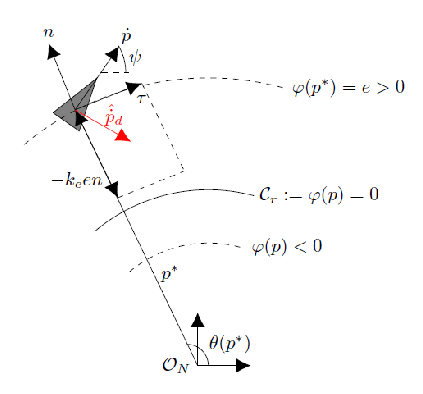
\includegraphics[width=0.55\textwidth]{figures/Control_1_2.eps}
\caption{Ejemplo de convergencia de un vehículo a la formación circular destino [referencia]} \label{Primera_Acción_Control}
\end{figure}

Posteriormente, se debe definir una trayectoria circular de radio $D\in\mathbb{R}^+$ puede ser descrita mediante la siguiente ecuación:
\begin{equation}
	C_D\triangleq\left\lbrace{p:\varphi{\left(p\right)}=0}\right\rbrace{,}
\end{equation}

En donde, $\varphi\left(p\right)=p_{x}^{2}+p_{y}^{2}-r^{2}$ y $p=\left[p_x\hspace{2mm}p_y\right]^T$ que representa la posición cartesiana con respecto a un marco de coordenadas cuyo origen esta en el centro de $C_D$. Este pertenece al espacio $\mathbb{C}^2$ y este es regular para cualquier posición exceptuando en el centro, es decir, $\nabla{\varphi\left(p\right)}\neq{0}\Longleftrightarrow{p}\neq{0}$ y todo el conjunto de niveles $\varphi_c\left(p\right)$ se pueden parametrizar. Si se particulariza para cada vehículo i se puede obtener dicha parametrización asociada a su posición mediante:

\begin{equation}
	\theta_{i}\left(p\right)=atan2\left(p_{x},p_{y}\right)\in\left(-\pi,\pi\right]
\end{equation} 

Adicionalmente, se describen dos vectores para el funcionamiento del algoritmo. El primero de ellos se atribuye a un vector normal a la circunferencia dada por $\varphi\left(p\right)$ definiéndose como $n\left(p\right)\triangleq\nabla\varphi\left(p\right)$, el otro es un vector tangente al punto $p$ y descrito por $\tau\left(p\right)=E\cdot{n\left(p\right)}$ con $E = \bigl[\begin{smallmatrix}0 & 1\\ -1 & 0\end{smallmatrix}\bigr]$ una matriz de rotación de $-\frac{\pi}{2}$.

Para cumplir el primero de los objetivos propios del algoritmo descritos en el principio de esta sección se debe considerar el siguiente modelo no holonómico. \footnote[3]{Sistema físico cuyo estado depende del camino tomado para lograrlo.}

\begin{equation}
	 \left \{
    \begin{aligned}
\dot{p}_{i}=u_{r}\cdot{m\left(\psi_{i}\right)}\\
\dot{\psi_{i}}=u_{\psi_{i}}\hspace{5mm}\\
    \end{aligned}
  \right.
\end{equation}

En donde, $u_{r}$ es la velocidad que ha de ser constante, además de tener el mismo valor para cada uno de los vehículos, $m=\left[\cos\left(\psi_{i}\right)\hspace{2mm}\sin\left(\psi_{i}\right)\right]^{T}$ con $\psi_{i}$ siendo el angulo de guiñada \footnote[4]{En este problema es igual al de ángulo de orientación} y $u_{\psi_{i}}$ es el parámetro con el que se consigue el control, obteniendo la convergencia de cada USV hacia la formación circular deseada. Este ultimo se encuentra definido como:

\begin{equation} \label{Action_Control}
	u_{\psi}=-\left(E\cdot\hat{\dot{p_d}}\cdot{\hat{\dot{p_{d}^{T}}}}\cdot{E}\left(\left(E-k_{e}\cdot{e}\right)\cdot{H\left(\varphi\right)}\cdot{\dot{p}}-k_{e}\cdot{n^T}\cdot{\dot{p}}\cdot{n}\right)\right)^{T}\cdot{E}\cdot{\frac{\dot{p_d}}{\|\dot{p_{d}}\|^{2}}}+k_{d}\cdot{\hat{\dot{p_{d}}}}\cdot{E}\cdot{\hat{\dot{p_{d}^{T}}}}
\end{equation}

Los detalles de la obtención de dicha expresión se pueden consultar en [referencia]. En donde, $H\left(\cdot\right)$ es el hessiano, $k_{d}\in\mathbb{R}^{+}$ es una constante que altera la velocidad de convergencia \footnote[5]{Describiendo una exponencial.} con la que cada vehículo viaja en torno a $c_D$ y $\hat{\dot{p_{d}}}$ es el campo vectorial que ha de seguir el vehículo. Este se define:

\begin{equation} \label{Control_for}
	\hat{\dot{p_{d}}}\triangleq\tau\left(p\right)-k_{e}\cdot{e\left(p\right)}\cdot{n\left(p\right)},
\end{equation}

En esta $k_{e}\in\mathbb{R}^{+}$ es una ganancia que define cuan agresivo es el campo vectorial para converger a $C_D$ y $e\left(p\right)\triangleq\varphi\left(p\right)$ es el error en la distancia entre el vehículo y la circunferencia objetivo. 

Con toda esta información se puede observar en la figura \ref{Primera_Acción_Control} un ejemplo de la aplicación de la ecuación \ref{Control_for} y la acción de control \ref{Action_Control}, es decir, se tiene un vehículo cualquiera en el plano cartesiano el cual ha de ser capaz de converger mediante $\hat{\dot{p_{d}}}$ en el que se conocen en todo momento: la componente normal $n$ y tangencial del vehículo $\tau$, su posición en el plano descrita por $\varphi\left(p\right)$ \footnote[6]{La notación que posee un * se corresponde con coordenadas respecto al eje del propio vehículo.} y finalmente su ángulo de orientación $\psi$. 

Un comentario destacable es que si el radio  descrito por el vehículo fuese menor que el deseado el lado derecho de la ecuación \ref{Control_for} se volvería positivo conllevando a que dicho vector apunte en la dirección contraria a la ilustrada en la figura \ref{Primera_Acción_Control}.\\

\begin{figure}[htb]
\centering
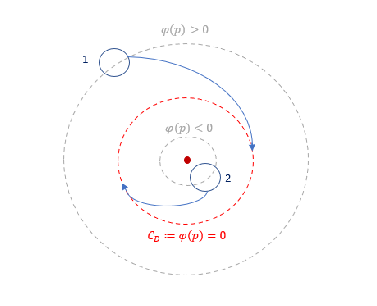
\includegraphics[width=0.62\textwidth]{figures/Pruea_Coordinacion.eps}
\caption{Ejemplo de disposición simétrica en torno a la formación circular} \label{Ejemplo_Coordinacion}
\end{figure}
\newpage
Una vez descrita la capacidad de convergencia asociada a cada vehículo se introduce la capacidad de disponerse uniformemente en torno a la formación circular. Para ello se dispone de la velocidad angular definida para cada uno de los vehículos:

\begin{equation}
	\dot{\theta}_{i}=\frac{u_{r}}{r}
\end{equation}

En donde, $u_{r}$ es la velocidad lineal que ha de ser constante como se describió al principio de la sección y $\dot{\theta}_{i}$ \footnote[7]{$\dot{\theta}_{i}=\frac{d\theta}{dt}=\omega_{i}$} es la velocidad angular asociada a cada vehículo.

La idea es controlar el ángulo entre vehículos $z = B^{T}\theta$ modificando la trayectoria descrita. Se define:

\begin{equation}\label{Control}
	C_i\left(D,c_{i}\right)\triangleq\left\lbrace{p:\varphi\left(p\right)=c_{i}}\right\rbrace
\end{equation}

En donde, $c_i \in \mathbb{R}$ es la señal de control de formación y el subindice $i\in\mathcal{V}$ denota cada uno de los vehículos. A partir de dicha ecuación surgen dos situaciones:

\begin{itemize}
	\item Si $c_i$ se hace muy pequeño, el radio D tenderá a aumentar y con ello se reduce la velocidad angular $\dot{\theta}_i$. Situación del agente 1 en la figura \ref{Ejemplo_Coordinacion}
	\item Si $c_i$ se hace muy grande, el radio D tenderá a disminuir y con ello se aumenta la velocidad angular $\dot{\theta}_i$. Situación del agente 2 en la figura \ref{Ejemplo_Coordinacion}
\end{itemize}

Se define a $c_i\triangleq{^{i}u}_{D}^{2}+2D\cdot{^i}u_{D},$ donde $^{i}u_{D}\in\mathbb{R}$ es una acción de control que posee un significado físico más directo al imponer el radio de la circunferencia de la siguiente forma:

\begin{equation}
	x^2+y^2-r^2={^{i}}u_{D}^{2}+2D{^{i}}u_{D} \Leftrightarrow x^2+y^2-(r+{^{i}}u_{D})^2
\end{equation}

La acción de control adquiere el siguiente significado ${^{i}}{u}_{D}=k_{r}\sum_{i=1}^N{B_i}\cdot{e}$, definiendo a $B_i$ como cada una de las filas de la matriz de incidencia \ref{Incidence}, $k_r\in\mathbb{R}^{+}$ y $e$ se corresponde con el error de formación descrito como: 

\begin{equation} \label{Error_Coordinacion}
	e_{\theta_{k}}\left(t\right)=z_{k}\left(t\right)-z_{k}^{*}
\end{equation}

En donde $e_{\theta_{k}}\in\left(-\pi,\pi\right]$ con $k\in\left\lbrace{1,\cdots,|\mathcal{E}|}\right\rbrace$. Definiendo como objetivo final del algoritmo que cuando $t\rightarrow\infty$ se tenga que $e_{\theta}\rightarrow{0}$ y $p_{i}\left(t\right)\rightarrow{C_D}$, en otras palabras, que pasado un tiempo el error sea el mínimo posible permitiendo que cada uno de los vehículos este dispuesto uniformemente a lo largo de la circunferencia. Esto se traduce en que la diferencia entre el ángulo entre vehículos real y el deseado se minimice. Finalmente, se impone sobre $k_{r}$ la condición de $r-\pi\cdot{k_{r}}max\left(\left\lbrace\mathcal{N}_{i}\right\rbrace\right)>0$. Esta impide la posibilidad de tener radios negativos en \ref{Control}.

\section{Algoritmo de ascenso de gradiente}

Hasta el momento únicamente se ha comentado sobre la cooperación de los agentes para la disposición de una figura geométrica y simétrica requerida o un algoritmo para la estima del gradiente en un punto. No obstante, se ha dejado de lado el avance de los agentes, es decir, ha de existir un algoritmo que desplace a todo el enjambre hacia la ubicación de la fuente haciendo uso del gradiente estimado.

Para ello, se utiliza el algoritmo de ascenso de gradiente su objetivo principal es desplazar el centro de la formación circular dado que sobre este se encuentra definido el gradiente, la ecuación que lo describe presenta la siguiente forma \cite{Adicional_Estimacion_1}:

\begin{equation}\label{GA}
	c_{k+1}=c_k+\epsilon\cdot\nabla{f}\left(c_k\right)\hspace{10mm}c_k=[x,y]\hspace{2mm}\forall_{x,y}\in\mathbb{R}
\end{equation}

En donde, $c_k$ corresponde con el centro de la formación circular y $\epsilon\in\mathbb{R}^{+}$. Al tratarse de un problema definido como un punto máximo de una función, el avance ha de ser estrictamente positivo, es decir, los valores han de ser cada vez mayores para desplazarte hacia dicho punto.

\section{Operación conjunta de los tres algoritmos.}

\begin{figure}[htb]
\centering
\includegraphics[width=0.75\textwidth]{figures/Flujo2.eps}
\caption{Diagrama de flujo que describe la dinámica del sistema.} \label{fig:Flujo}
\end{figure}
\newpage
En la figura \ref{fig:Flujo} se pueden apreciar diferentes colores para diferenciar cada uno de los pasos a seguir antes de que los USVs lleguen a la zona con máximas sustancias contaminantes, desglosándolos estos serían:

\begin{enumerate}
	\item Se disponen los N agentes en el plano, es decir, se conoce la posición de cada uno de los USV en la superficie marítima.
	\item Se ejecuta el algoritmo de control de formación circular para hacer que convergan cada uno de los vehículos a la formación circular y a su vez se dispongan de manera simétrica. Un aspecto a destacar es que se tiene que poner un umbral para decidir cuando avanzar. Dicho umbral esta estrictamente relacionado con el error de la formación, es decir, si este valor es lo suficientemente pequeño el enjambre avanza; en caso contrario, se quedarán esperando a que todos los agentes se coloquen en sus sitios. 
	\item Al ya estar dispuestos en la circunferencia, se hace la estimación del gradiente para su valor en el centro de la formación. En este punto, se dan dos casos que en la figura \ref{fig:Flujo} están referidos como A:
	\begin{itemize}
		\item Si $\widehat{\mathrm{\nabla }}{f}\left(c_{k}\right)\approxeq0$ se está cerca de la fuente conformando una \textbf{solución satisfactoria}.
		\item Si $\widehat{\mathrm{\nabla }}{f}\left(c_{k}\right)>0$ aun están desplazándose para llegar al objetivo.
	\end{itemize}
	\item En caso de darse la segunda de las situaciones antes planteadas, se ha de desplazar el centro de la formación circular mediante el algoritmo de ascenso de gradiente mediante la ecuación \ref{GA}.
	\item Antes de volver a estimar el gradiente se debe comprobar el paso 2, en caso de permanecer cada uno de los agentes en la formación y el error es lo suficientemente pequeño, se pasa directamente al paso 3.
\end{enumerate}








